\documentclass[../em.tex]{subfiles}
\graphicspath{{\subfix{../figures/}}}
\begin{document}
\chapter{Electric Circuits}
\section{Electric Current}
Current is the rate at which charge passes through a cross-sectional area of a wire.
\[I=\mathrm{d}q/\mathrm{d}t \implies q = \int I \mathrm{d}t\]
Current within a conductor consists charge carriers traveling through the conductor with an average drift velocity.
\[I=nqv_D A\]
Electric charge moves in a circuit in response to an electron potential difference, sometimes referred to as electromotive force, or emf ($\epsilon$)

Current density if the flow of charge per unit area.
\[I=\int{\vec{J}\cdot\mathrm{d}\vec{A}} \implies I = JA\]
Current density is related to the motion of the charge carriers within a conductor and is a vector quantity.
\[J=nqv_D\]
A potential difference across a conductor creates an electric field within the conductor that is proportional to the resistivity and the current density.
\[\vec{E}=\rho \vec{J}\]
If a function of current density is given, the total current can be determined by integrating the density over the area.
\[I=\int \vec{J(r)}\cdot\mathrm{d}\vec{A}\]gg6
Although current is a scalr quantity, it does have direction.
\begin{itemize}
    \item The direction of conventional current is chosen to be the direction in which positive charge would move.
    \item In common circuits, the current is actually due to the movement of electrons.
\end{itemize}

\begin{example}
    A long conducting cylinder has radius $R$, and carries a current to the left. The current density varies with distance 
    $r$ from the cylinder's central axis according to the equation $J=kr^2$, where $r\leq R$ and $k$ is a positive constant. Derive an expression
    for the total current in the cylinder.

    \begin{align*}
        I=\int\vec{J}(r)\cdot\mathrm{d}\vec{A} \\
        = \int (kr^2)(2\pi r\mathrm{d}r)
        = \frac{\pi k}{2}R^4
    \end{align*}
\end{example}

\section{Simple Circuits}
A circuit is composed of electrical loops, which can include wires, batteries, resistors, 
lightbulbs, capacitors, inductors, switches, ammeters, and voltmeters.

A closed electrical loop is a closed path through which charges may flow.
\begin{itemize}
    \item A closed circuit is one in which charges would be able to flow.
    \item An open circuit is one in which charges would not be able to flow.
    \item A short circuit is one which charges would be able to flow with no change in potential difference.
\end{itemize}

Circuit schematics are representations used to describe and analyze electric circuits.
\begin{itemize}
    \item The properties of an electric current are dependent on the physical arrangement of its constituent elements.
\end{itemize}
Circuit elements have common symbols that are used to create schematic diagrams.
\begin{itemize}
    \item If an element is variable, then the element is indicated by a diagonal strikethrough arrow across the symbol.
\end{itemize}
\begin{center}
    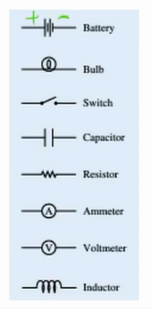
\includegraphics[width=0.2\textwidth]{appc111.PNG}
\end{center}
\section{Ohm's Law and Electrical Power}
\begin{itemize}
    \item Resistance is a measure of the degree to which an object opposes the movement of electrical charge.
    \item It is proportional to its resistivity and length and is inversely proportional to its cross-sectional area.
    \[R=\frac{\rho l}{A}\]
    \item This assumes the resistivity to be uniform.
    
    \item If the resistivity is not uniform, meaning it varies along the length, use:
    \[R=\int{\frac{\rho(l)}{A}}\mathrm{d}l\]

    \item Ohm's Law relates current, resistance, and potential difference across a conductive element of current.
    \[I=\frac{\Delta V}{R}\implies V = IR\]

    \item The resistivity of an ohmic material is constant regardless of temperature.
    
    \item The resistance of an ohmic circuit element can be determined from the slope of a graph of the current in the element as a function of the potential difference across the element.
    \item The rate at which energy is transferred, converted or dissipated by a circuit element depends on the current in the element and the electrical potential difference across it.
    \item The brightness of a lightbulb increases with power, so power can be used to qualitatively predict the brightness of lightbulbs in a circuit.
\end{itemize}
\section{Compound Direct Current Circuits}
Circuit elements may be connected in series and/or parallel.

A series connection is one in which any charge passing through one circuit element must proceed through all elements in that connection and has no other path available.

The current in each series circuit element is the same.

A parallel connection is one in which chargesm ay pass through one of two or more paths.

Across each path, the potential difference is the same.

Ideal batteries and wires have negligible internal resistance.

If the battery is not ideal, then it has an internal resistance.
\[\Delta V_{\text{Terminal}}=\epsilon - IR \]
Ammeters are used to measure current at a specific point in a circuit. It must be connected in series in the circuit.

Voltmeters are used to measure the electric potential difference between two points in a circuit. They must be connected in parallel.
\section{Kirchoff's Rules}
\begin{itemize}
    \item Kirchoff's Rules quantify how current flows through a circuit and how voltage varies around a loop in a circuit.
    \item Kirchoff's Loop Rule is a consequence of the conservation of energy.
    \begin{itemize}
        \item This is sometimes called Kirchoff's Voltage Law.
        \item It states that the sum of the potential differences across all circuit elements in a single closed loop must equal zero.
        \[\sum V + 0\]
    \end{itemize}
    \item Kirchoff's Junction Rule is a consequence of the conservation of charge.
    \begin{itemize}
        \item This is sometimes called Kirchoff's Current Law.
        \item It states the total amount of charge entering a junction per unit time must equal the total amount of charge exiting the junction per unit time.
        \[\sum I = 0\]
    \end{itemize}
\end{itemize}

\section{Resistor-Capacitor (RC) Circuits}
A collection of capacitors in a circuit may be analyzed as though it was a single capacitor with an equivalent capacitance $C_{ep}$.

As a result of conservation of charge, each of the capacitors in series must have the same magnitude of charge on each plate.

The charge on a capacitor or the current in a resistor in a RC circuit can be described by a 
fundamental differential equation derived from Kirchoff's loop rule.
\[ \epsilon = \frac{\dd q}{\dd t}R+\frac{q}{C} \]

The time constant ($\tau$) is a significant feature of an RC circuit.

The time constant of an RC circuit is a measure of how quickly the capacitor will charge or discharge and is defined as 
\[\tau = RC\]
\end{document}